%compile with writelatex.com
\documentclass[a4paper]{article}
\usepackage[english]{babel}
\usepackage[utf8]{inputenc}
\usepackage{amsmath}
\usepackage{graphicx}
\usepackage{epigraph}%for quotes
%\epigraphfontsize{\small\itshape}
\setlength\epigraphwidth{1\textwidth}
\setlength\epigraphrule{0pt}
\usepackage[colorinlistoftodos]{todonotes}
\usepackage{color}
\usepackage{hyperref}
\usepackage{float}
\usepackage{fancyhdr}
\usepackage{sidecap}%enables figcap next to picture for larger captions
\usepackage[yyyymmdd,hhmmss]{datetime}%for generating auto time stemp
%from geogebra
\usepackage{pstricks-add}
\usepackage{pgf,tikz}
\usetikzlibrary{arrows}
\newrgbcolor{xdxdff}{0.49 0.49 1}
\newrgbcolor{uququq}{0.25 0.25 0.25}
\newrgbcolor{vvvvvv}{0.33 0.33 0.33}
\newrgbcolor{ayayay}{0.66 0.66 0.66}
\newrgbcolor{srsrsr}{0.13 0.13 0.13}
\definecolor{qqwuqq}{rgb}{0.13,0.13,0.13}
\definecolor{uququq}{rgb}{0.25,0.25,0.25}
\definecolor{xdxdff}{rgb}{0.66,0.66,0.66}
\definecolor{qqqqff}{rgb}{0.33,0.33,0.33}
\newcommand{\degre}{\ensuremath{^\circ}}
\psset{xunit=1.0cm,yunit=1.0cm,algebraic=true,dotstyle=o,dotsize=3pt 0,linewidth=0.8pt,arrowsize=3pt 2,arrowinset=0.25}
%end from geogebra
\renewcommand{\deg}{\ensuremath{^{\circ}}}%enable degree symbol for angles and celcius
\pagestyle{fancy}
\newcommand{é}{\'e}
\newcommand{ë}{\"e}
%edit this if you need a different date
\newcommand{\todayDate}{\today}
\rfoot{Compiled on \todayDate\ at \currenttime GMT}
\cfoot{}
\lfoot{Page \thepage}


\begin{document}
\begin{titlepage}
    \centering

	\title{Dictaat Medium Coeli\\*
		$\in$\\*
		college ascendantberekening\\*
		\small
		$\in$\\*
		colleges\\*
		$\subset$\\*
		Concrete meetkunde}
	\author{\href{http://svlentink.co.nf}{Sander Lentink} \small F131999 \\*
		\small
        	\href{http://wiskuu.nl}{Mathematisch Instituut},
            \href{http://uu.nl}{Universiteit Utrecht},
            the Netherlands}

	\date{\todayDate}

\maketitle
\thispagestyle{empty}%remove pagenumber on title page

\Huge $M^c$

%http://patentimages.storage.googleapis.com/WO1999000781A1/imgf000062_0001.png
\includegraphics[width=.7\textwidth]{basic.png}

\epigraph{"Once you understand the magnetic line of energy between the MC/IC axis you will understand
the energy that shaped your inner-self (id) and outer-self (ego)."}{---
\href{http://marianneohagan.com/astrology/asc-dec-axis-and-mc-ic-axis/the-mc-ic-axis}{Marianne O'Hagan}}

%\\[4in]
\scriptsize - The pdf version of this document contains hyperlinks. -

\end{titlepage}

\newpage

\tableofcontents

\newpage

\section{Introduction}

The midheaven (MC or Medium Coeli, literally 'middle of the sky') is one of the most important angles used in
\href{http://en.wikipedia.org/wiki/Natal_astrology}{Natal astrology},
also known as genethliacal astrology.
Astrologers believe that each individual's personality or path in life can be determined by constructing a natal chart for the moment and location of that individual's birth.
They believe that the midheaven will tell you about your
career, status, aim in life, aspirations, public reputation, and life goal.
\\
\\
Since astrology is a \textbf{pseudoscience}, I won't discuss the meaning or background.
This document is aimed at the mathematical aspect of the midheaven.
In the back you'll find a copied chapter about the meaning (interpretation by astrologer) of the signs.

%generated my personal natal chart and converted the gif to jpg
%login as quest user on: http://www.astro.com/cgi/chart.cgi?btyp=w2at&rs=3
\begin{figure}[H]
\centering
\includegraphics[width=1\textwidth]{natal.jpg}
\caption{\label{natal}Natal chart}
\end{figure}

Notice that we are looking at astrology, not astronomy.
Astrology is the divination by the stars, astronomy is the scientific study of the stars.


\newpage


\section{\href{http://www.math.nus.edu.sg/aslaksen/projects/kh-urops.pdf}{Basics}}

This chapter contains all the basics, needed to understand the concept.

\subsection{Projective geometry}
Astrology works with projective geometry.
Everything you see is projected onto an imaginary sphere.
This means that we do not look at the distances of the celestial bodies,
only to their relative positions on the
\href{http://en.wikipedia.org/wiki/Celestial_sphere}{celestial sphere}.
I.e. we look at the angular differences, as seen from the Earth.


%http://astrobob.areavoices.com/files/2011/11/North-pole-diurnal-1024x505.jpg
\begin{figure}[H]
\centering
\includegraphics[width=.9\textwidth]{zenith.jpg}
\caption{\label{zenith}Celestial sphere with zenith}
\end{figure}

\subsection{\href{http://en.wikipedia.org/wiki/Celestial_sphere}{Celestial sphere}}

We can project all the celestial bodies we see onto an imaginary dome.
This dome is spread out over the observer, who is at the centre of the dome.
This is a way of modeling how the
%This is one of the ways to model how the
\href{http://google.com/sky}{sky}
appears to us.
Notice that in reality, the celestial bodies do have various distance from the Earth.
We however don't need that for calculating the midheaven.

\subsection{Zenith}

The zenith is like a normal (geometry), it is the point on the celestial sphere overhead of an observer on Earth.

\newpage

%http://nd03.jxs.cz/849/352/a65205cacc_88238970_o2.jpg
\begin{figure}[H]
\centering
\includegraphics[width=.5\textwidth]{horizons.jpg}
\caption{\label{horizons}Example of wrong horizons}
\end{figure}

\subsection{Horizon}

The celestial sphere has $\infty$ many
\href{http://en.wikipedia.org/wiki/Great_circle}{great circles}.
We want the horizon to be a great circle.
In order to be able to do this, we need to make the celestial sphere large enough,
so we can neglect the angular difference and take the horizon as a plane through the centre of the earth.

The horizon cuts the celestial sphere into two equal halves, with one visible to the observer.
We call this the "ground level" of the observer.


\subsection{Celestial poles}

The celestial sphere rotates around an axis.
This axis provides us with the north and south celestial poles (NCP and SCP).

%http://physics.weber.edu/schroeder/ua/CelestialSphere.png
\begin{figure}[H]
\centering
\includegraphics[width=.5\textwidth]{CelestialSphere.png}
\caption{\label{celestialPoles}Celestial poles viewed from observer}
\end{figure}

\subsection{Celestial equator}

When we observe the terrestrial equator, we can draw a plane on it,
passing through the centre of the earth.
When we would extend this plane, it would also pass through the celestial sphere,
creating the celestial equator.
This celestial equator lies between the celestial poles.

\newpage

\subsection{Meridian}\label{meridian_chap}

All places on earth are on a
\href{http://en.wikipedia.org/wiki/Meridian_(geography)}{meridian}
(line of longitude).
Greenwich is chosen as 0\deg, everything east ranges from 0 to 180, and west from 0 to -180.
Geography works with east and west, we'll use $\lambda \in (-180,180)$ for the math.
Utrecht is located 5\deg east of Greenwich.

The central meridian (meridian of observer) is an imaginary arc which passes from the north point on the horizon to the south, passing through the zenith.
\\
\\
Notice that everywhere on the meridian, the location of east and west are the same.
This makes that the great circle of
\textbf{the celestial equator, intersects with the horizon (also a great circle) in the west and east}
at all times.


\subsection{Ecliptic}

%http://star-www.st-and.ac.uk/~fv/webnotes/chapter9.htm
%http://star-www.st-and.ac.uk/~fv/webnotes/SEASONS.GIF
\begin{figure}[H]
\centering
\includegraphics[width=.8\textwidth]{seasons.jpg}
\caption{\label{seasons}Seasons (helocentric perspective)}
\end{figure}

Looking from the geocentric perspective,
the ecliptic is the annual path of the sun, with respect to the stars.

This path is a great circle on the celestial sphere.
The plane, drawn on the ecliptic, makes an angle of
\href{https://www.google.com/search?q=what+is+the+angle+of+the+ecliptic}{$\approx 23.4\deg$}
($23\frac{1}{2}\deg$ is widely used) with the (celestial) equator.

This tilt is responsible for the seasons on Earth.

%http://star-www.st-and.ac.uk/~fv/webnotes/chapter9.htm
%http://star-www.st-and.ac.uk/~fv/webnotes/eclipt1.GIF
\begin{figure}[H]
\centering
\includegraphics[width=1\textwidth]{sine.jpg}
\caption{\label{sine}Sine function}
\end{figure}

To see this on Google, search for:
\href{https://www.google.com/search?q=graph+23.4*sin(x*2pi%2F365)}{"graph 23.4*sin(x*2pi/365)"}
\\
\\
It is important to understand this concept.
Here are some simulations which can help you get a better understanding:
\\
\small \href{http://astro.unl.edu/classaction/animations/coordsmotion/eclipticsimulator.html}{http://astro.unl.edu/classaction/animations/coordsmotion/eclipticsimulator.html}
\\
\small \href{http://astro.unl.edu/classaction/animations/coordsmotion/sunmotions.html}{http://astro.unl.edu/classaction/animations/coordsmotion/sunmotions.html}
\\
\small \href{http://astro.unl.edu/classaction/animations/coordsmotion/sunsrays.html}{http://astro.unl.edu/classaction/animations/coordsmotion/sunsrays.html}


\newpage


%http://www.astro.virginia.edu/class/skrutskie/images/ecliptic0.jpg
%\begin{figure}[H]
%\centering
%\includegraphics[width=.8\textwidth]{equinox.jpg}
%\caption{\label{equinox}Equinox}
%\end{figure}

%https://dept.astro.lsa.umich.edu/ugactivities/Labs/precession/ecl_equ_prec.jpg
\begin{figure}[H]
\centering
\includegraphics[width=1\textwidth]{precession.jpg}
\caption{\label{precession}Precession circle}
\end{figure}

\subsection{Equinoxes and Solstices}

It is given that two great circles on a sphere intersect at two points,
these points are diametrically opposite to each other.
\\
\\
The intersecting points of the ecliptic and celestial equator are called equinoxes.
There is a vernal equinox (spring) which fall on
\href{https://www.google.com/search?q=vernal+equinox}{$\approx$ March 20},
and a autumnal equinox which falls on
\href{https://www.google.com/search?q=a+autumnal+equinox}{$\approx$ September 23}.
At these equinoxes, the night and day are of equal length.
\\
\\
The solstices are the shortest and longest day of the year.
The longest day falls on
\href{https://www.google.com/search?q=what+is+the+summer+solstice}{$\approx$ June 21}
and the shortest on
\href{https://www.google.com/search?q=what+is+the+winter+solstice}{$\approx$ December 22}.

\newpage

%http://static.comicvine.com/uploads/original/10/101779/2542084-tattoo_pictures_of_zodiac_signs_scorpio_zodiac_tattoo_designs.jpg
%\begin{figure}[H]
%\centering
%\includegraphics[width=.7\textwidth]{zodiac.jpg}
%\caption{\label{zodiac} Zodiac}
%\end{figure}

%http://www.hko.gov.hk/gts/time/calendarinfoimages/image003e.gif
\begin{figure}[H]
\centering
\includegraphics[width=.93\textwidth]{zodiacInfo.jpg}
\caption{\label{zodiac}Zodiac, divided into 12 parts of $\frac{360}{12} = 30\deg$}
\end{figure}


\subsection{Zodiac}

The zodiac is a division of the
\href{http://google.com/sky}{sky}
into twelve parts.
Each part has its own sign, starting with Aries.
The zodiac plane is drawn on the ecliptic plane.
The vernal equinox is the starting point, commonly denoted by V (referring to the Aries sign).

%http://7promeniv.com.ua/7rays_psychology/03_7RaysScience/Astrology/Education_Programm/Velykiy_Maliy_Zodiack.files/image006.jpg
\begin{figure}[H]
\centering
\includegraphics[width=.5\textwidth]{zodiacBelt.jpg}
\caption{\label{zodiacBelt}Zodiac on ecliptic}
\end{figure}



\newpage



\section{Sidereal time}

The time we use is based on our observation of the sun (solar time).
The Earth rotates around its axis in about 24h.

The sidereal time involves the stars, the sky;
we are looking for the rotation of the celestial sphere.

The Earth rotates around the sun in $365\frac{1}{4}$ days (calendar year).
Because the Earth rotates around the sun and around its own axis, the sidereal time,
the time to have the vernal equinox on the same point, is $366\frac{1}{4}$ days.

To understand this concept, look at it this way:
from a geocentric perspective;
the sun appears to move, relative to the stars, around the Earth once per year.
This results in one fewer solar day per year.
\\
\\
This means that a point in space, e.g. Aries sign, will be on the same meridian
every

\begin{equation}\label{sid_equ}
\frac{365.2422}{366.2422} = 0.99726956642
\end{equation}

day, or 23 hours, 56 minutes and 4 seconds.

\subsection{Greenwich}

Greenwich Mean Time (GMT) is what we will use to calculate the sidereal time.
\\
Every year, around March 20 at noon, the meridian of Greenwich, and the vernal equinox
(intersection of the ecliptic and celestial equator) intersect.

\subsection{(Sidereal) hour angle}

When the vernal equinox is on an observer's meridian,
we say that the Local Sidereal Time (LST) is 0 hours.
After 23h, 56m and 4s, the hour angle is again 0.
The LST is the angle between the vernal equinox and the local meridian.
So, LST = Local Hour Angle (LHA) of the vernal equinox.
(this hour angle plane is drawn onto the ecliptic)


\subsection{History}\label{historySDT}

To calculate the siderial time, you need to know the GMT.
Different places on Earth have different time zones.
Some have DST (daylight savings time), others don't.
\\
\scriptsize * Different locations have different starting and ending of DST.
\\
\\
\normalsize For example, the germans (WWII) forced the Netherlands to use CET (Central European Time),
this is used since May 16, 1940.
\\
From Sep. 16, 1945 to Apr. 3, 1977, the Netherlands did not have DST.
\\
\\
This are only two facts to consider when calculating for such a small country.
The reader is responsible to find the correct information, matching his location and date.


\subsection{Example}\label{example}
June 10, 1991, 7.56AM, Lelystad, Netherlands;
\\
Lelystad is located in the CET time zone, GMT+1.
Also, DST was active; GMT+2.
This means that the GMT time at that moment was 5.56AM.


\newpage


\subsection{Calculation}\label{calculation}

\textbf{Step 1}, finding the GMT time.
For June 10, 1991, 7.56AM we found 5.56AM.
\\
It's up to the reader to find the correct time, as explained in chapter \ref{historySDT}
\\
\\
\textbf{Step 2}, we know that around March 20 at noon the vernal equinox intersects with the meridian.
So, we now going to
\href{http://www.timeanddate.com/date/durationresult.html?d1=20&m1=3&y1=1991&d2=10&m2=6&y2=1991&h1=12&i1=0&s1=0&h2=5&i2=56&s2=0}{calculate}
how much days have been past since that moment.
\scriptsize For easy calculation: \href{http://www.timeanddate.com/date/durationresult.html?d1=20&m1=3&y1=1991&d2=10&m2=6&y2=1991&h1=12&i1=0&s1=0&h2=5&i2=56&s2=0}{timeanddate.com/date/durationresult.html}
\\
\normalsize For our example date and time (using 5.56, not 7.56) we get 81 days, 17 hours and 56 minutes.
\\
\\
Side note; for a more precise calculation,
look for the vernal equinox date and time on the year you're searching for.
(it's not March 20 at noon precise)
\\
\\
\textbf{Step 3}, converting to days only.

\begin{equation}
d + \frac{1}{24}(h + \frac{m}{60})
\end{equation}

For our example this results in
\href{http://www.wolframalpha.com/input/?i=81+%2B+%281%2F24%29%2817+%2B+56%2F60%29}{$81 + \frac{1}{24}(17 + \frac{56}{60}) = 81.7472$}
days.
\\
\\
\textbf{Step 4}, to get the sidereal days,
we multiply this by the difference found by equation \ref{sid_equ} (notice that we use the reciprocal).

\begin{equation}
( d + \frac{1}{24}(h + \frac{m}{60}) ) \cdot \frac{366.2422}{365.2422}
\end{equation}

This result will give us the amount of sidereal days since March 20 at noon.
Which means, the amount of rotations of the vernal equinox.
For our example this results in
\href{http://www.wolframalpha.com/input/?i=%2881+%2B+%281%2F24%29%2817+%2B+56%2F60%29%29*%28366.2422%2F365.2422%29}{$(81 + \frac{1}{24}(17 + \frac{56}{60})) \cdot \frac{366.2422}{365.2422} = 81.9710$}
sidereal days.
\\
\\
\textbf{Step 5}, for the MC we want to know the angle on the zodiac (which lies on the ecliptic).
To get this we need to know where the vernal equinox is (the 0\deg point).
\\
\\
When looking at the sidereal days, we only need the decimal part (the whole days are whole rotations, which result in the same point).

\begin{equation}
( (d + \frac{1}{24}(h + \frac{m}{60})) \cdot \frac{366.2422}{365.2422} ) \mod{1}
\end{equation}

To convert to an angle, we multiply it by 360\deg.

\begin{equation}
( ( (d + \frac{1}{24}(h + \frac{m}{60})) \cdot \frac{366.2422}{365.2422} ) \mod{1} ) \cdot 360\deg
\end{equation}

Seen from Greenwich, our example would be 0.971 sidereal day.
\\
\href{http://www.wolframalpha.com/input/?i=%28%28%2881+%2B+%281%2F24%29%2817+%2B+56%2F60%29%29*%28366.2422%2F365.2422%29%29mod1%29*360}{$( ( (81 + \frac{1}{24}(17 + \frac{56}{60})) \cdot \frac{366.2422}{365.2422} ) \mod{1} \cdot ) 360\deg = 350\deg = 0.971 * 360\deg $}
\\
\\
\textbf{Step 6}, you're probably not in Greenwich, or on its meridian.
We use the longitude $\lambda \in (-180,180)$, as we have seen in chapter \ref{meridian_chap},
to correct for the fact that we're on a different meridian.

\begin{equation}
\href{http://www.wolframalpha.com/input/?i=%28%28%28d+%2B+%281%2F24%29%28h+%2B+m%2F60%29%29*%28366.2422%2F365.2422%29%29mod1%29*360+%2B+%CE%BB}{( ( (d + \frac{1}{24}(h + \frac{m}{60})) \cdot \frac{366.2422}{365.2422} ) \mod{1} ) \cdot 360\deg + \lambda}
\end{equation}

For our example, Lelystad, $\lambda = +5\deg$. Which gives us $350\deg + 5\deg = 355\deg$.


\newpage


%http://zakeiaben.wikispaces.com/file/view/%60.gif/269818840/%60.gif
\begin{figure}[H]
\centering
\includegraphics[width=.8\textwidth]{sunsPath.jpg}
\caption{\label{sunsPath}The text "celestial dome" can be seen as meridian}
\end{figure}


\section{Midheaven}

Midheaven or medium coeli (MC) is an important aspect of natal astrology.
Together with the ascendant or "rising sign" (intersection ecliptic and horizon) in the east
(where the sun rises), and the decendant (intersection ecliptic and horizon) in the west.
\\
\\
The MC lies in between the ascendant and decendant,
it's the middle of the sky, which is, for a given observer on his meridian.
So, to calculate the MC, we look at the intersection of the ecliptic and the meredian.
\\
\\
Notice that we're not looking for the location of the sun, but the annual path of the sun.
Also, the MC sign for a given siderial time is the same for the whole meridian (regardless of latitude).


\subsection{Imum Coeli}

The IC, Imum Coeli (Latin for "bottom of the sky"), lies opposite to the MC.
When we have found the MC, we look 180\deg further on the zodiac to find the IC.



\newpage



\section{Spherical trigonometry}

\begin{figure}[!h]
\centering
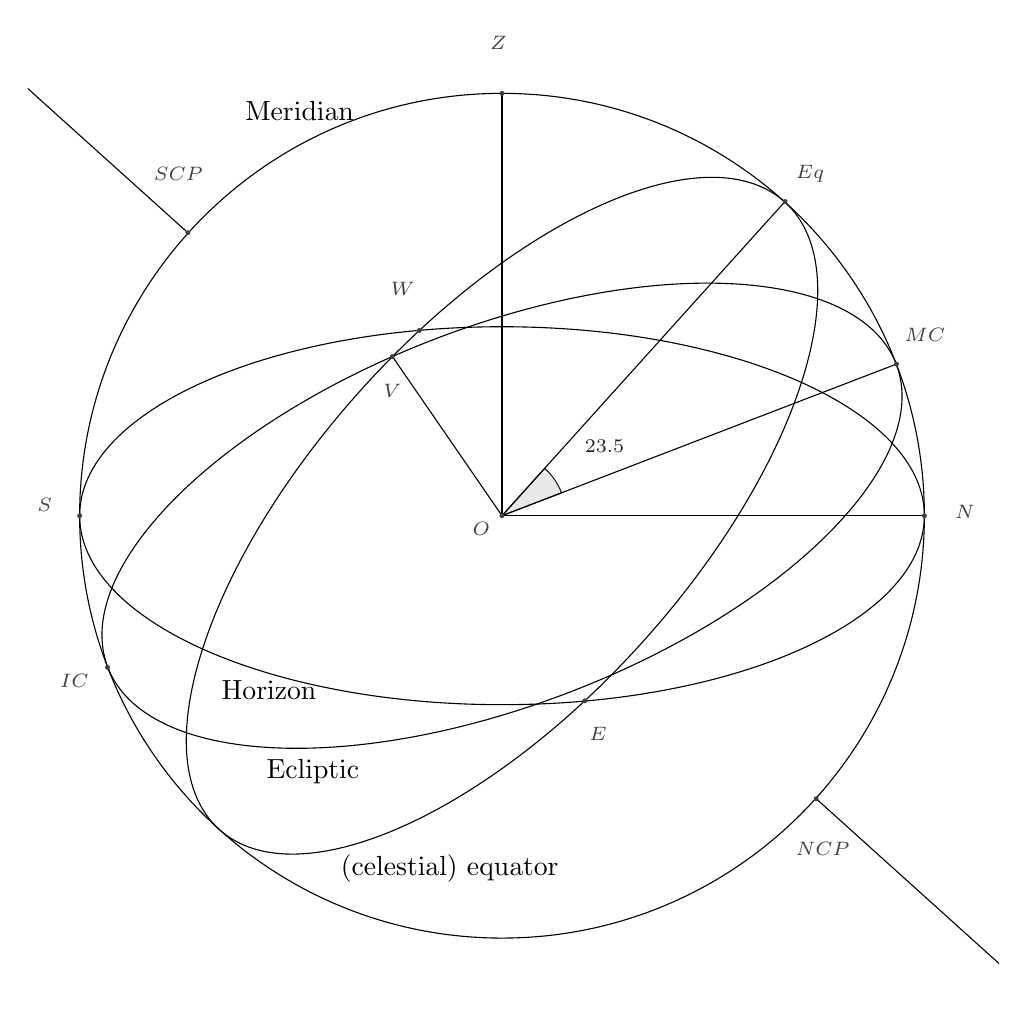
\begin{tikzpicture}[line cap=round,line join=round,>=triangle 45,x=1.0cm,y=1.0cm,scale=.6]


\clip(-10.04,-9.87) rectangle (10.52,10.33);
\draw [shift={(0,0)},color=qqwuqq,fill=qqwuqq,fill opacity=0.1] (0,0) -- (21.04:1.35) arc (21.04:47.98:1.35) -- cycle;
\draw [rotate around={0:(0,0)}] (0,0) ellipse (8.94cm and 4cm);
\draw(0,0) circle (8.94cm);
\draw [rotate around={47.98:(0,0)}] (0,0) ellipse (8.94cm and 4cm);
\draw [rotate around={21.04:(0,0)}] (0,0) ellipse (8.94cm and 4cm);
\draw (0,0)-- (0,8.94);
\draw (0,0)-- (5.99,6.65);
\draw (0,0)-- (8.35,3.21);
\draw (0,0)-- (8.94,0);
\draw (-6.14,-3.28) node[anchor=north west] {Horizon};
\draw (-5.19,-4.94) node[anchor=north west] {Ecliptic};
\draw (-3.62,-6.96) node[anchor=north west] {(celestial) equator};
\draw (-2.32,3.37)-- (0,0);
\draw (-5.64,8.98) node[anchor=north west] {Meridian};
\draw (-6.65,5.99)-- (-16.32,14.7);
\draw (6.65,-5.99)-- (16.29,-14.68);
\begin{scriptsize}
\fill [color=uququq] (0,0) circle (1.5pt);
\draw[color=uququq] (-0.44,-0.27) node {$O$};
\fill [color=uququq] (-8.94,0) circle (1.5pt);
\draw[color=uququq] (-9.68,0.23) node {$S$};
\fill [color=uququq] (0,8.94) circle (1.5pt);
\draw[color=uququq] (-0.08,10.01) node {$Z$};
\fill [color=uququq] (8.94,0) circle (1.5pt);
\draw[color=uququq] (9.8,0.09) node {$N$};
\fill [color=uququq] (1.75,-3.92) circle (1.5pt);
\draw[color=uququq] (2.03,-4.62) node {$E$};
\fill [color=uququq] (-1.75,3.92) circle (1.5pt);
\draw[color=uququq] (-2.1,4.8) node {$W$};
\fill [color=uququq] (-2.32,3.37) circle (1.5pt);
\draw[color=uququq] (-2.32,2.65) node {$V$};
\draw[color=qqwuqq] (2.17,1.48) node {23.5};
\fill [color=uququq] (-6.65,5.99) circle (1.5pt);
\draw[color=uququq] (-6.85,7.23) node {$SCP$};
\fill [color=uququq] (6.65,-5.99) circle (1.5pt);
\draw[color=uququq] (6.79,-7.05) node {$NCP$};
\fill [color=uququq] (5.99,6.65) circle (1.5pt);
\draw[color=uququq] (6.52,7.23) node {$Eq$};
\fill [color=uququq] (8.35,3.21) circle (1.5pt);
\draw[color=uququq] (8.95,3.82) node {$MC$};
\fill [color=uququq] (-8.35,-3.21) circle (1.5pt);
\draw[color=uququq] (-9.05,-3.5) node {$IC$};


\end{scriptsize}
\end{tikzpicture}
%\caption{\label{trigonometry} \small $M_{eq}$ = intersection meridian and equator,
%$M_{ec}$ = intersection meridian and ecliptic}
\end{figure}

When we look at figure above, we see the three great circles, needed to calculate a natal chart.
For a given place, we know its longitute and latitude,
and the angle between the ecliptic and equator is known.
\\
\\
As we have seen in chapter \ref{calculation}, we can calculate the hour angle of the ecliptic plane.
We know that the ecliptic and equator intersect on point V.
The earth rotates around the earth's axis,
which means that the sidereal time tells us where point V is on the \textbf{equator}.
%I.e. the angle on the ecliptic plane between point V and point $M_{EC}$, $\angle VOM_{EC}$.
In the example above, this would be around 100\deg.
(The sun comes up at the east, traveling to the west.
We start at the meridian, from which we measure the angle.)
\\
\\
%For calculating the ascendant, we need the triangle, formed between the west point,
%point V and the ascendant (intersection horizon and ecliptic).
%This is done by finding where V lies on the ecliptic plane (see chapter \ref{calculation}).
%In the example above, this gives us $|WV| = 100-90=10\deg$.
%The $\angle ZOM_{eq}$ is found by the using the latitude, from which we can find angle W of the triangle.
%Together with the angle between the ecliptic and the equator
%($\angle V = 23.5\deg$) we are were able to calculate the ascendant.


\newpage


The MC (midheaven) for a given sidereal time will remain the same regardless of the latitude of the location.
In other words, this variable latitude, is obsolete.
\\
For the given example (chapter \ref{example}) we get:

%http://astro.unl.edu/classaction/animations/coordsmotion/sunmotions.html?t=5.56&d=10&m=june&lat=52.5
\begin{SCfigure}%[H]
\centering
\includegraphics[width=.5\textwidth]{picForJune10.png}
\caption{\label{picForJune10}\href{http://astro.unl.edu/classaction/animations/coordsmotion/sunmotions.html?t=5.56&d=10&m=june&lat=52.5}{5.56AM, June 10, lat = 52.5\deg}
\*
Yellow (which we do not use) = sun's declination (its daily path),
\*
white = the ecliptic (sun's annual path),
\*
blue = celestial equator (other blue = prime hour circle or 0h right ascension)
\*
It is important to
\textbf{notice that the equator and meridian will always make a 90\deg angle.}}
\end{SCfigure}

\begin{figure}[!h]
\centering
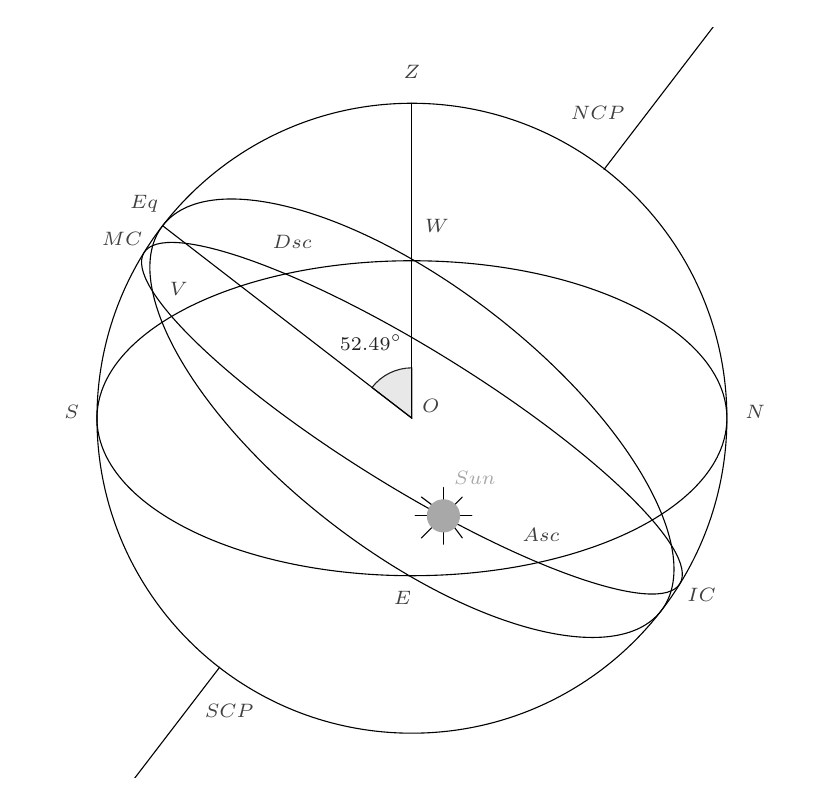
\begin{tikzpicture}[line cap=round,line join=round,>=triangle 45,x=1.0cm,y=1.0cm,scale=4]


\clip(-1.22,-1.14) rectangle (1.2,1.24);
\draw [shift={(0,0)},color=qqwuqq,fill=qqwuqq,fill opacity=0.1] (0,0) -- (90:0.16) arc (90:142.49:0.16) -- cycle;
\draw(0,0) circle (1cm);
\draw (-0.61,-0.79)-- (-4.54,-5.92);
\draw (0.61,0.79)-- (3.59,4.68);
\draw [rotate around={0:(0,0)}] (0,0) ellipse (1cm and 0.5cm);
\draw [rotate around={-37.7:(0,0)}] (0,0) ellipse (1cm and 0.42cm);
\draw (0,0)-- (-0.79,0.61);
\draw [rotate around={-31.72:(0,0)}] (0,0) ellipse (1cm and 0.22cm);
\draw (0,1)-- (0,0);
\draw(0.1,-0.31) circle (0.04cm);
\draw (0.1,-0.27)-- (0.1,-0.22);
\draw (0.07,-0.28)-- (0.03,-0.25);
\draw (0.05,-0.31)-- (0.01,-0.31);
\draw (0.07,-0.34)-- (0.03,-0.38);
\draw (0.1,-0.35)-- (0.1,-0.4);
\draw (0.13,-0.34)-- (0.16,-0.38);
\draw (0.14,-0.31)-- (0.19,-0.31);
\draw (0.13,-0.28)-- (0.16,-0.25);
\begin{scriptsize}
%\fill [color=uququq] (0,0) circle (1.5pt);
\draw[color=uququq] (0.06,0.04) node {$O$};
\draw[color=qqwuqq] (-0.13,0.24) node {$52.49\textrm{\degre}$};
%\fill [color=uququq] (-1,0) circle (1.5pt);
\draw[color=uququq] (-1.08,0.02) node {$S$};
%\fill [color=uququq] (1,0) circle (1.5pt);
\draw[color=uququq] (1.09,0.02) node {$N$};
%\fill [color=uququq] (0.61,0.79) circle (1.5pt);
\draw[color=uququq] (0.59,0.97) node {$NCP$};
%\fill [color=uququq] (-0.61,-0.79) circle (1.5pt);
\draw[color=uququq] (-0.58,-0.93) node {$SCP$};
%\fill [color=uququq] (0,0.5) circle (1.5pt);
\draw[color=uququq] (0.08,0.61) node {$W$};
%\fill [color=uququq] (0,-0.5) circle (1.5pt);
\draw[color=uququq] (-0.03,-0.57) node {$E$};
%\fill [color=uququq] (-0.85,0.53) circle (1.5pt);
\draw[color=uququq] (-0.92,0.57) node {$MC$};
%\fill [color=uququq] (-0.82,0.4) circle (1.5pt);
\draw[color=uququq] (-0.74,0.41) node {$V$};
%\fill [color=uququq] (0.4,-0.46) circle (1.5pt);
\draw[color=uququq] (0.41,-0.37) node {$Asc$};
%\fill [color=uququq] (-0.4,0.46) circle (1.5pt);
\draw[color=uququq] (-0.38,0.56) node {$Dsc$};
%\fill [color=uququq] (-0.79,0.61) circle (1.5pt);
\draw[color=uququq] (-0.85,0.68) node {$Eq$};
%\fill [color=uququq] (0,1) circle (1.5pt);
\draw[color=uququq] (0,1.1) node {$Z$};
\fill [color=xdxdff] (0.1,-0.31) circle (1.5pt);
\draw[color=xdxdff] (0.2,-0.19) node {$Sun$};
%\fill [color=uququq] (0.85,-0.53) circle (1.5pt);
\draw[color=uququq] (0.92,-0.56) node {$IC$};


\end{scriptsize}
\end{tikzpicture}
\caption{\label{PersonalTrigonometry} \small Picture for example seen in \ref{example}
(52.5\deg = latitude Lelystad)}
\end{figure}


We see $\triangle Eq,MC,V$ with $\angle MC,Eq,V = \frac{\pi}{2} = 90\deg$.


\newpage


\begin{figure}[!h]
\centering
\begin{tikzpicture}[line cap=round,line join=round,>=triangle 45,x=1.0cm,y=1.0cm,scale=14]


\clip(6.73,13.63) rectangle (7.26,14);
\draw [shift={(7.77,7.2)},color=qqwuqq,fill=qqwuqq,fill opacity=0.1] (0,0) -- (161.49:0.06) arc (161.49:180:0.06) -- cycle;
\draw [shift={(7.18,13.87)},color=qqwuqq,fill=qqwuqq,fill opacity=0.1] (0,0) -- (180:0.06) arc (180:203.5:0.06) -- cycle;
\draw [domain=6.73:7.26] plot(\x,{(-7.2-0*\x)/-1});
\draw(8.68,10.64) circle (3.56cm);
\draw (6.48,7.84)-- (6.48,7.2);
\draw (6.48,7.2)-- (7.77,7.2);
\draw (6.85,13.87)-- (6.85,13.69);
\draw (6.85,13.87)-- (7.18,13.87);
\begin{scriptsize}
\fill [color=qqqqff] (6.48,7.2) circle (1.5pt);
\draw[color=qqqqff] (8.43,12.19) node {$M_{EC}$};
\fill [color=qqqqff] (8.68,10.64) circle (1.5pt);
\draw[color=qqqqff] (9.27,12.21) node {$F$};
\fill [color=uququq] (6.48,7.84) circle (1.5pt);
\draw[color=uququq] (8.47,12.22) node {$M_{eq}$};
\fill [color=uququq] (7.77,7.2) circle (1.5pt);
\draw[color=uququq] (8.71,12.23) node {$V_1$};
\draw[color=black] (7.14,7.18) node {6\textrm{\degre}};
\fill [color=xdxdff] (7.34,7.35) circle (1.5pt);
\draw[color=xdxdff] (8.62,12.23) node {$A$};
\draw[color=qqwuqq] (8.53,12.2) node {23.5};
%\fill [color=qqqqff] (6.85,15.09) circle (1.5pt);
\draw[color=qqqqff] (8.5,13.97) node {$H$};
%\fill [color=qqqqff] (4.16,13.87) circle (1.5pt);
\draw[color=qqqqff] (6.77,13.61) node {$I$};
%\fill [color=uququq] (6.85,13.87) circle (1.5pt);
\draw[color=uququq] (6.81,13.91) node {$Eq$};
%\fill [color=uququq] (6.85,13.69) circle (1.5pt);
\draw[color=uququq] (6.81,13.72) node {$MC$};
%\fill [color=uququq] (7.18,13.87) circle (1.5pt);
\draw[color=uququq] (7.2,13.84) node {$V$};
%\fill [color=qqqqff] (-11.6,5.7) circle (1.5pt);
\draw[color=qqqqff] (6.77,12.73) node {$J$};
\draw[color=qqwuqq] (7.05,13.85) node {$23.5\textrm{\degre}$};


\end{scriptsize}
\end{tikzpicture}
\caption{\label{personalTriangle} Triangle for the given example, see figure \ref{picForJune10}}
\end{figure}

$|AC| = b =$ siderial time,
\\
$|AB| = c =$ what we are looking for


\begin{figure}[!h]
\centering
\begin{tikzpicture}[line cap=round,line join=round,>=triangle 45,x=1.0cm,y=1.0cm,scale=14]


\clip(6.73,13.63) rectangle (7.26,14);
\draw [shift={(7.77,7.2)},color=qqwuqq,fill=qqwuqq,fill opacity=0.1] (0,0) -- (161.49:0.06) arc (161.49:180:0.06) -- cycle;
\draw [shift={(7.18,13.87)},color=qqwuqq,fill=qqwuqq,fill opacity=0.1] (0,0) -- (180:0.06) arc (180:203.5:0.06) -- cycle;
\draw [domain=6.73:7.26] plot(\x,{(-7.2-0*\x)/-1});
\draw(8.68,10.64) circle (3.56cm);
\draw (6.48,7.84)-- (6.48,7.2);
\draw (6.48,7.2)-- (7.77,7.2);
\draw (6.85,13.87)-- (6.85,13.69);
\draw (6.85,13.87)-- (7.18,13.87);
\begin{scriptsize}
\fill [color=qqqqff] (6.48,7.2) circle (1.5pt);
\draw[color=qqqqff] (8.43,12.19) node {$M_{EC}$};
\fill [color=qqqqff] (8.68,10.64) circle (1.5pt);
\draw[color=qqqqff] (9.27,12.21) node {$F$};
\fill [color=uququq] (6.48,7.84) circle (1.5pt);
\draw[color=uququq] (8.47,12.22) node {$M_{eq}$};
\fill [color=uququq] (7.77,7.2) circle (1.5pt);
\draw[color=uququq] (8.71,12.23) node {$V_1$};
\draw[color=black] (7.14,7.18) node {6\textrm{\degre}};
\fill [color=xdxdff] (7.34,7.35) circle (1.5pt);
\draw[color=xdxdff] (8.62,12.23) node {$A$};
\draw[color=qqwuqq] (8.53,12.2) node {23.5};
%\fill [color=qqqqff] (6.85,15.09) circle (1.5pt);
\draw[color=qqqqff] (8.5,13.97) node {$H$};
%\fill [color=qqqqff] (4.16,13.87) circle (1.5pt);
\draw[color=qqqqff] (6.77,13.61) node {$I$};
%\fill [color=uququq] (6.85,13.87) circle (1.5pt);
\draw[color=uququq] (6.83,13.87) node {$C$};
%\fill [color=uququq] (6.85,13.69) circle (1.5pt);
\draw[color=uququq] (6.84,13.66) node {$B$};
%\fill [color=uququq] (7.18,13.87) circle (1.5pt);
\draw[color=uququq] (7.2,13.84) node {$A$};
%\fill [color=qqqqff] (-11.6,5.7) circle (1.5pt);
\draw[color=qqqqff] (6.77,12.73) node {$J$};
\draw[color=qqwuqq] (7.05,13.85) node {$23.5\textrm{\degre}$};


\end{scriptsize}
\end{tikzpicture}
\caption{\label{triangleABC} Important: $\gamma$ needs to be 90\deg}
\end{figure}



We use the formulas, given in "dictaat Bolmeetkunde", page 11 (lectured by Prof. J.P. Hogendijk).
We'll just give the formulas without proving them, the formulas with the known variables (b, $\alpha$) are:

\begin{enumerate}
\item $\cos \alpha = \cos a \cdot \sin \beta$
\item $\cos \beta = \cos b \cdot \sin \alpha$ $\surd$
\item $\sin \alpha = \frac{\sin a}{\sin c}$
\item $\sin \beta = \frac{\sin b}{\sin c}$
\item $\cos \alpha = \frac{\tan b}{\tan c}$ $\surd$
\item $\tan \alpha = \frac{\tan a}{\sin b}$ $\surd$
\item $\tan \beta = \frac{\tan b}{\sin a}$
\end{enumerate}


\newpage



%To find $|BC|$ we use formula 6:

%\begin{multline}
%\tan \alpha = \frac{\tan a}{\sin b}
%\Rightarrow
%\tan 23.5\deg = \frac{\tan |BC|}{\sin sidereal}
%\Leftrightarrow
%\\
%\tan |BC| = \tan sidereal \cdot \tan 23.5\deg
%\end{multline}

To find $c$ we use formula 5:

\begin{multline}\label{form5}
\cos \alpha = \frac{\tan b}{\tan c}
\Rightarrow
\cos 23.5\deg = \frac{\tan sidereal}{\tan c}
\Leftrightarrow
\\
\tan c = \frac{\tan sidereal}{\cos 23.5\deg}
\end{multline}

%To find $\angle EC$ we use formula 2:

%\begin{equation}
%\cos \beta = \cos b \cdot \sin \alpha
%\Rightarrow
%\cos \angle EC = \cos sidereal \cdot \sin 23.5\deg
%\end{equation}


%http://what-is-astrology.com/img/ZodiacRuler.gif
\begin{figure}[H]
\centering
\includegraphics[width=.5\textwidth]{basicZodiac.jpg}
\caption{\label{basicZodiac}Basic zodiac, see figure \ref{zodiac} for a full version}
\end{figure}


\subsection{Final}

On calculator:
\href{http://www.wolframalpha.com/input/?i=tan%5E-1%28tan%285%29%2Fcos%2823.5%29%29}{
$\tan^{-1}(\frac{\tan 5}{\cos 23.5})$}

For our example we have sidereal = 5\deg
(not 355, see figure \ref{picForJune10}),
using equation \ref{form5} we obtain
\href{http://www.wolframalpha.com/input/?i=tan%5E-1%28tan%285%29%2Fcos%2823.5%29%29}{5.5\deg}.
Looking at figure \ref{PersonalTrigonometry}, we see that we need to look in the other direction.

This shows us that the MC is in Pisces.
\\
$ -5.5\deg + 360\deg = 354.5$, and $354.5 \mod 30 = 24.5\deg$ tells us that it's 24.5\deg Pisces.
\\
\\
To find the IC, just add 180\deg, this gives us 24.5\deg Virgo

\newpage

\subsection{Another example}

%generated my personal natal chart and converted the gif to jpg
%login as quest user on: http://www.astro.com/cgi/chart.cgi?btyp=w2at&rs=3
\begin{figure}[H]
\centering
\includegraphics[width=1\textwidth]{jan.png}
%\caption{\label{natal2}Natal chart}
\end{figure}

Given: 21 July 1955, 8:30AM, Leeuwarden (53\deg12'N 5\deg47'E)
\\
Looking at the cheat sheet (chapter \ref{cheatsheet}) we get $\lambda = +5.78\deg$ (+; because east of Greenwich)
\\
\\
Looking at chapter \ref{calculation}:
\\
\textbf{Step 1}, DST in July: normally yes, but chapter \ref{historySDT} tells us no. CET = GMT+1; 7:30AM.
\\
\textbf{Step 2},
\href{http://www.timeanddate.com/date/durationresult.html?d1=20&m1=3&y1=1991&d2=21&m2=7&y2=1991&h1=12&i1=0&s1=0&h2=7&i2=30&s2=0}{122 days, 19 hours and 30 minutes.}
\\
\textbf{Step 6},

\begin{equation}
\href{http://www.wolframalpha.com/input/?i=%28%28%28122+%2B+%281%2F24%29%2819+%2B+30%2F60%29%29*%28366.2422%2F365.2422%29%29mod1%29*360+%2B+5.78}{( ( (122 + \frac{1}{24}(19 + \frac{30}{60})) \cdot \frac{366.2422}{365.2422} ) \mod{1} ) \cdot 360\deg + 5.78\deg = 59.33\deg}
\end{equation}


\newpage


Next, visualization using:
\scriptsize \href{http://astro.unl.edu/classaction/animations/coordsmotion/sunmotions.html}{http://astro.unl.edu/classaction/animations/coordsmotion/sunmotions.html}
\normalsize

%http://astro.unl.edu/classaction/animations/coordsmotion/sunmotions.html
\begin{figure}[H]
\centering
\includegraphics[width=.5\textwidth]{janSun.png}
\caption{\label{janSun}\href{http://astro.unl.edu/classaction/animations/coordsmotion/sunmotions.html}{7:30AM, July 21, lat = 53\deg}}
\end{figure}

On calculator:
\href{http://www.wolframalpha.com/input/?i=tan%5E-1%28tan%2859%29%2Fcos%2823.5%29%29}{
$\tan^{-1}(\frac{\tan 59}{\cos 23.5})$}

For this example we have sidereal = 59\deg,
using equation \ref{form5} we obtain
\href{http://www.wolframalpha.com/input/?i=tan%5E-1%28tan%2859%29%2Fcos%2823.5%29%29}{61\deg}.
Looking at figure \ref{janSun}, we see that we look in the normal direction.

This shows us that the MC is 1\deg in Gemini,
and the IC is 1\deg Sagittarius.


\newpage


\section{Cheat sheet: time to decimals}\label{cheatsheet}

Since we have already seen this in previous lectures I'll just give an example.
\\
\\
What we need to know:

\begin{itemize}
\item 1 h = 1\deg = 60' (min)
\item 1' (min) = $\frac{1}{60}$h = $\frac{1}{60}$\deg = 60" (sec)
\item 1" (sec) = $\frac{1}{60}$' (min)
\end{itemize}

\subsection{Time example}

Given: 12\deg27'15"

\begin{enumerate}
\item 15" (sec) $\cdot \frac{1}{60} = 0.25$' (min)
\item 27' + 0.25' = 27.25' (min)
\item 27.25' (min) $\cdot \frac{1}{60} = 0.4541666\deg$ (h)
\item $12\deg + 0.4541666\deg = 12.454167\deg$ (h)
\end{enumerate}

\subsection{Decimal example}

Given: 12.454167\deg

\begin{enumerate}
\item 12\deg (h)
\item $0,454167\deg \cdot 60 = 27.25002$' (min)
\item 27' (min)
\item $0.25002' \cdot 60 = 15.0012$" (sec)
\item 12\deg27'15"
\end{enumerate}









\newpage

\section{\href{http://marianneohagan.com/astrology/asc-dec-axis-and-mc-ic-axis/the-mc-ic-axis}{Meaning}}\label{meaning}

\subsection{MC ARIES - IC LIBRA}
As a child you may have tried to avoid confrontational situations; you tended to follow rather than lead. You may have been ‘passive’ or you felt you were ‘singled out’ or ‘set apart’ from others which may have affected your ‘social expression. Perhaps you felt you had to separate yourself from others to keep the peace, and to find your own way to ‘self-sufficiency’. In your primary years, constant aggressive confrontations may have interfered with your ability to assert yourself and your individual rights. You had a tendency to ‘cower’ from aggressive behaviour through the continuing social conflicts of your childhood. Peace and harmony in all relationships was important to you; this was hard to uphold, but you did your best to keep the peace because you felt more secure in peaceful surroundings. When you were older you challenged yourself to become independent, to become ‘your own person’; you wanted to make your own way in the world. Due to a certain ‘lack of self-confidence’, you may have felt that you did not have the skills, or the ability to make it in the world, so you ‘put your head down’, looked inward and found the ‘strength’ to become ‘self-sufficient’ and ‘independent’. Your focus on the world is one of ‘self-reliance’ and ‘independence’. You prefer to be ‘your own boss’; you will try to place yourself in ‘sole-charge’ positions of ‘your own making’ rather than working for someone else. In public you try to project an image of light-hearted humour which helps other people to ‘lighten up’, and in their light-hearted laughter you feel happy and fulfilled.

\subsection{MC TAURUS - IC SCORPIO}
To get love you looked for approval and if you didn’t get it - it hurt. You needed encouragement but you were kept under very strong dominance or control within the family; there was only one way,’ ‘their way’. You felt you didn’t belong or you didn’t get along with a sibling. Your parents had a powerful influence and effect on you; they may have manipulated your behaviour to accommodate their arrangements or affairs. You could have felt emotionally removed or separated from a parent in some way – maybe the death or distancing of a parent which may have left you feeling insecure. The psychological effect of your childhood was deep; trust may have been broken which may have affected future relationships. You may have felt unwanted and unattractive, that you couldn’t show your true self. You need to look inwards to resolve subconscious childhood issues in order to gain emotional security. You were taught the value of money because financial undertones were issues, yet the financial situation was never discussed. You were provided for but you may have felt the least important person; ‘kept down’ which may have led to a basic feeling of insecurity. When you matured you felt you couldn’t depend on anyone else, you had to depend on yourself. In order to overcome the insecurity you felt in ‘self’ you needed to become financially independent; to land on your ‘own two feet’. You will work at achieving financial security through your own rules, but with a strong work ethic. You are non-materialistic, you will make do. You like to give to other people in practical or material ways, but you can be ‘ripped off’ easily. You will give ‘things’ to people (‘things’ to you are just ‘things’) but if what you give to others makes them happy, then you feel happy too; however you can give too much away.

\newpage

\subsection{MC GEMINI - IC SAGITTARIUS}
As a child you may have lacked confidence through the lectures, reprimands and corrections from a strict parent who had a handle on everything and whose words were ‘law’; however the truth was often twisted and comments were made. You were made to feel guilty through family members or other people’s opinions and judgements. One of your parents may have placed high expectations on you, or judged your behaviour either negatively or positively due to the inconsistencies of your childhood. Unfair conclusions may have been used against you where you felt you had to justify yourself. You did your best to succeed at school but you may have felt your efforts were not always recognised by your teachers and/or your parents. You may have experienced misrepresentation in your childhood, but from this you learned to respect the truth. You have a tendency to question the ‘so-called’ truth in any debatable situation where you ‘know’ that the version of the truth is manufactured. You are a deep thinking person with good communication skills and you like to share your opinions on a wide range of topics and philosophies that are thought provoking. When you help people with their problems, you listen to them; then offer a wide range of alternatives from a philosophical angle that gives them faith in the future. You guide others through their problems in an intelligent and positive way. You strive to find the truth in any situation and you need to ‘know’ the truth in order to make judgement. You have a ‘many-faceted mind’ and you take all angles into consideration before you reach a conclusion. You open up new vistas of thought, and you offer alternatives when helping others. You enjoy solving other people’s problems, and when you succeed, you feel inwardly fulfilled and good about yourself. You judge situations based on truth and fact to reach fair and just conclusions.

\subsection{MC CANCER - IC CAPRICORN}
As a child you were shy and cautious in your approach. Your parents set the example and they disciplined you, they expected you to take responsibility and trusted you to do things correctly. You may have had fears of failing your parents; you wanted to please them in order to gain approval. You could have blamed yourself when family conflicts arose, with a tendency to withdraw. Family conflicts may have played on your feelings of inner control and security. Recognition was hard to gain in many areas due to family disciplines and standards. You may have felt distanced from some family members; perhaps you had little contact with cousins or relatives. Family disciplines were exercised through family business and/or family burdens. Your mother was very important to you but you may have felt your emotional needs were not met. You could have felt distanced from a parent who was either absent or worked very hard. You may have longed for the care and support of family involvement, but instead you may have felt an inner sense of isolation. You respected your parents, and you were disciplined – incorrect behaviour met with disapproval. You may have felt that others were recognised ahead of you; or that others could express themselves better than you; maybe if you expressed yourself, you would not be approved of; providing you were good, you were safe – this could have affected your ‘self-esteem’. Your parents encouraged you to be self-supporting and encouraged you to work at a young age; the work provided may have been organised through your family. The world is your family but public concerns can dominate your private life and you can concern yourself over other people’s positions and values. Your approach to other people is one of consideration and welfare. You understand the need for basic support and security and you care about the emotional needs of other people. You try to guide others towards their own security by giving them the tools to use in that which they are aiming for. By helping them you feel inwardly fulfilled. Your feelings run deep and you want to ‘make things better’ for the people who approach you in order to reduce their anxieties and uncertainties. You will try to help them get what they want, to make their lives more comfortable. You feel good about yourself when you help other people find their own security.

\subsection{MC LEO - IC AQUARIUS}
As a child you could have been quietly, or openly rebellious (depending on the sign on the Ascendant) if you did not get the freedom you needed to express yourself. You played with friends in the neighbourhood and people may have visited your home. You were taught to treat everyone as equal. You may have associated with a child, or a sibling who was ‘different’ in some way; through this you developed understanding and humanitarianism. In your growing-up years, you could have felt ‘different’ from your friends. Your parents may have had totally different personalities – they were diverse. One parent may have been anti-social and the other social; and you were given the space to develop your social skills independently. You have many friends, and you probably relate well to their problems, but you may feel inwardly separate, somewhat detached and possibly ‘different’. You can lack faith in yourself through a feeling of neglect in love, and an inner fear of being ‘hurt’; therefore you may detach from love to protect your feelings. As an adult you may choose not to make close friends outside your personal circle, preferring to be independent; some may consider you aloof, but you tend to set yourself apart from ‘collective’ social groups; however you mix well with people from all walks of life and you do not cast judgement on class, race or creed. You try to help other people to succeed, and if they do, their success gives you an inner sense of pride. When you are with your selected friends, you are lively, colourful and entertaining. You enjoy fun and entertainment, and you meet with interesting friends from different backgrounds. You try to encourage your partner to share your interests, but this can be an area of social difference.

\subsection{MC VIRGO - IC PISCES}
As a child you were sensitive and imaginative. One of your parents was an idealist who tried to create an ideal family situation. You may have felt as if that parent was ungrounded, but you could have idealised them anyway. Family issues may have been swept under the carpet because nasty things were not spoken of; therefore situations built up to the point of explosion.
Conflicts between your parents were not voiced so you did not know what was required of you. When the family needs were not met, one of your parents could desensitise and become less loving because you had not done what was expected of you. You had your duties, and you were expected to carry them out, which you did in your own time. You may have been considered untidy because one of your parents had very high expectations and you felt you had to live up to them. You were expected to be quiet and good, so it felt good to escape into a world of your own. With your childhood sensitivity and vivid imagination you could easily escape through reading and music, or any other form of creative expression. You were a very shy child, and you may have been afraid to join groups, preferring one-to-one relationships, yet you longed to join in with the fun of group involvement. As you grew older you became a realist; you could see escapism didn’t work. You had to develop your communication skills and gain confidence. You have a tendency to take on the role of ‘hard worker’ for your family. You may feel you have to pay the bills and take care of the general running of household duties. It can be difficult for you to allocate duties to other family members because you sacrifice in service for them. Your sensitivity to your family past, whether mental, physical or spiritual will manifest in your work ethics; and you will consider family needs ahead of your own. You will work hard to create an ideal family/home situation for your family, and you may consider it your duty to take responsibility for the welfare of your family.

\subsection{MC LIBRA - IC ARIES}
You could have been placed in a ‘take-charge’ position at a young age due to family circumstances, but this helped you to develop personal independence. You may have faced aggression in friendship in your primary years, but you learned to walk away from aggression and people who try to control you. You do not like to get involved in conflicts, but if you are pushed to your limit, you will break friendships that are not compatible. You do not like upheaval in your life, you like to balance relationships, and you tend to take the supportive role in friendship; this strengthens your friendships and relationships, and gives you a sense of inner satisfaction. In your childhood, you were exposed to issues of leadership (you had to learn to become independent). You either played the leading role, or you were led around by friends; from this you learned to balance relationships – ‘give and take’ equally. You are only too willing to help or support your friends; ‘you are there for them’ and you will ‘back them’ when they need you, but you believe in ‘equal sharing’ and ‘balanced relationships’; if relationships are not balanced, you will walk away. Relationships have to be on an ‘equal footing’; you are not dependent on others, and you are quite happy to be on your own. Although you enjoy socialising, you have a preference for one-to-one relationships. You show a charming and diplomatic face to the world and you have good ‘public relations’ skills; however if anyone tries to dominate your independence, you will exert your will and stand your ground on principle; you may have lost friends through this. When your relationships are based on equal sharing you feel good about yourself.

\newpage

\subsection{MC SCORPIO - IC TAURUS}
In your childhood secrets were withheld; this could have made you feel uncertain in the more secretive areas of family circumstance. You were not allowed to talk about issues involving private family concerns outside the family – family business was private and personal. Your mother supported you in school activities and outings, she created the family interests. These family interests can have accentuated the separate values of each family member resulting in a feeling of exclusion in matters that did not include you. Other people’s needs and values dominated, so you tended to help in support of their needs and values because you wanted to feel included and you usually did as you were asked. When everything is going right for those around you, you feel inwardly fulfilled, therefore you will try to give all the help and support you can to others. In public, you tend to wear a ‘mask’; you may feel that other people would not want to be with you if they knew the ‘inner you’. You keep your ‘ear to the ground’ because you suspect that other people can talk and you like to ‘know’ what is going on around you. You are sensitive to the environmental energy and you can pick up on the general tenor that exists beneath the surface in your surroundings, you need to ‘know’ that you are ‘accepted’ by those around you and that they are ‘happy with your involvement’. You may search for a deeper understanding behind the meaning of ‘life’ because you are consciously aware of the higher realms of existence which you seek to understand more deeply.

\subsection{MC SAGITTARIUS - IC GEMINI}
As a child, your parents did not mollycoddle you. You could have felt an island unto yourself, too shy to communicate, and in particular, at school. Perhaps you felt ‘little children should be seen and not heard’. You may have felt remote from your siblings. At school, you were shy, you did not speak up in class, and you did not make friends easily. You may have faced difficulty with education through a lack of stimulation, and you could have felt ostracised by some children; therefore primary school could have been a constrictive experience rather than a free-flowing one. You may have found it difficult to communicate with one of your parents who may have had different opinions from you which could have led to a lack of connection. You may have lost touch with some family members. As an adult you enjoy change, whether it is the house, the décor or the furniture; routine is boring and you are basically restless. Your inquisitive mind will drive you to study and obtain knowledge that can be useful in the outside world and you will inform and teach others through your own experience and knowledge. You are interested in learning about people across the board, but especially their origins and their life’s experiences. You help people through life’s experiences because you have a good understanding of the things that trouble most people. You are not pretentious in public; ‘what you see is what you get’ and you prefer to speak to people and not at them. You love to share any exciting knowledge you may have learned because you genuinely enjoy sharing new information and knowledge with others. You have a good sense of humour and you enjoy making other people laugh. You believe ‘laughter is the best medicine’ and you tend to look on the bright side of life.

\newpage

\subsection{MC CAPRICORN - IC CANCER}
As a child you were self-protective. You may have felt a lack of security over things you could not control which could have made you feel anxious. You were well provided for by your mother, but emotional or parental conflicts had a strong effect on you. Your relationship with your mother was sensitive or clinging; you needed to feel secure and protected, but often you felt your mother was not around, either physically or emotionally which could have made you feel anxious (especially if the MC is badly aspected in your chart) otherwise your childhood was well provided for. Worry over security and protection could have caused anxiety; you needed a peaceful environment, and you needed to feel a sense of ‘belonging’; to be part of the family. Should anything threaten that feeling, anxiety would be the result. Anxiety over family conflict may have disturbed you because you wanted everything to be calm, and family security was so very important to you. Your early childhood environment may have affected you on an emotional level, and this could have interfered with your ability to place your trust in close friendships and relationships. It was generally accepted that you would do well, and through this, you placed internal pressure on yourself to deliver. As you grew up, you gained a strong sense of having to build your own family structures, to move away from the past and take responsibility. Although you had a strong need for parental approval and respect, you came to realise that you could not lean on anyone else but yourself, and that you had to become self-sufficient. You try to encourage people to be the ‘best that they can be’. You build up other people’s confidence and ‘self-esteem’ which helps them realise their goals; then you feel happy and you release them. You acknowledge ‘ethically correct standards of conduct’ that you feel are correct for you.

\subsection{MC AQUARIUS - IC LEO}
As a child you were sociable and you tried hard to ‘fit in’ with your family. You craved affection but you may not have received as much affection as you wanted which could have led to feelings of insecurity. High expectations may have been placed on you and you were expected to act in a ‘proper manner’. ‘Social or class distinctions may have been an issue and this you may carry into your adult years. When you went out into the world you were friendly, but detached. You have your own personal interests and you prefer not to make friends with work associates. If work associates need you, you will support them and understand their needs, but once you have done this you will detach. You prefer to be independent. You recognise other people’s strengths and you will encourage and acknowledge them. You are a humanitarian and you work for the good of ‘people’. You don’t like undercurrents of ill feeling and discontent; you like to know what is wrong and you try to solve problems in a humanitarian way, but with straight talk. You treat all people equally; without ‘class distinction’. You are a humanitarian and you will defend, or help the underprivileged in society because you enjoy doing the ‘little things’ that count en masse for people. You take the time to listen to other people’s ‘woes’, and if you can ‘brighten up their day’, you feel good about yourself; this is all part of your helpfulness to humanity. You identify with people because ‘people are people’ and you are one of them; ‘do unto others as you would be done by’. You believe in equal rights and opportunity for all people and you play fair. Socio-economic ‘class’ and family values are strong, but you believe we are all equal and we should all get along in friendship and social equality.

\subsection{MC PISCES - IC VIRGO}
As a child you loved books and you enjoyed reading. You may have been exposed to family health issues in your growing-up years where one of your parents may have been associated with hospitals and/or healthcare, or had an interest in health issues such as healthy living, good food and good manners. You may have been at the mercy of family circumstances, but you developed humility and inner faith. You could have worried about issues of security, things that might happen, these things may have been non-specific, but they caused you to worry. Stress-related health conditions within the family could have given you the impression that you had to be good, and you did as you were told. One of your parents may have worried over small things, and could have suffered from stress-related illnesses. You tried to be quiet and not to upset anyone. Through family difficulties, you were expected to help, and you assumed childhood duties to reduce stress. You did this as a form of love and approval. You may have felt remote from a parent at some stage in your growing-up years. You developed a very deep understanding of what suffering was. You show sensitivity and compassion to those who are afflicted, whether through health conditions or social problems. You will empathise with them on a deep level to make them feel better. Your approach to the world is to alleviate the pain and suffering you see in society and through this you can feel spiritually uplifted.

\newpage

\section{References}

\subsection{Images}

\begin{description}
\item[Cover] http://patentimages.storage.googleapis.com/WO1999000781A1
%\item[Figure \ref{zodiac}] http://static.comicvine.com/uploads/original/10/101779
\item[Figure \ref{zenith}] http://astrobob.areavoices.com/files/2011/11/North-pole-diurnal-1024x505.jpg
\item[Figure \ref{horizons}] http://prvopodstata.blog.cz/1208/zakriveni-zeme
\item[Figure \ref{horizons}] http://nd03.jxs.cz/849/352
\item[Figure \ref{celestialPoles}] http://physics.weber.edu/schroeder/ua/CelestialSphere.png
\item[Figure \ref{seasons} \& \ref{sine}] http://star-www.st-and.ac.uk/~fv/webnotes/chapter9.htm
\item[Figure \ref{precession}] https://dept.astro.lsa.umich.edu/ugactivities/Labs/precession
\item[Figure \ref{zodiac}] http://www.hko.gov.hk/gts/time/calendarinfoimages/image003e.gif
\item[Figure \ref{zodiacBelt}] http://7promeniv.com.ua
\item[Figure \ref{sunsPath}] http://zakeiaben.wikispaces.com/file/view/%60.gif/269818840/%60.gif
\item[Figure \ref{picForJune10}] http://astro.unl.edu/classaction/animations/coordsmotion/sunmotions.html (values: t=5.56, d=10, m=june, lat=52.5)
\item[Figure \ref{basicZodiac}] http://what-is-astrology.com/img/ZodiacRuler.gif
\end{description}

\subsection{Internet}

%Special thanks to
%\href{http://www.math.nus.edu.sg/aslaksen/projects/kh-urops.pdf}{Kevin Heng Ser Guan},
%National University of Singapore, his document helped me to write this document.

\begin{description}
\item[Chapter \ref{meaning}] http://marianneohagan.com/astrology/asc-dec-axis-and-mc-ic-axis/the-mc-ic-axis
\item[Simulations] \href{http://astro.unl.edu/animationsLinks.html}{http://astro.unl.edu/animationsLinks.html}
\item[Verifier] \href{www.astro.com/cgi/chart.cgi?btyp=w2at&rs=3}{www.astro.com/cgi/chart.cgi?btyp=w2at\&rs=3}
\end{description}

\subsection{Literature}

\begin{description}
\item[Chapter \ref{historySDT}] Astrologische berekeningen, Ike Nagelkerke; page 39 
\end{description}


\end{document}
